\documentclass[a4paper,12pt]{book}
\usepackage[utf8]{inputenc}

\usepackage{rachwidgets}


\newcommand{\laClass}       {CS 211}
\newcommand{\laSemester}    {Spring 2018}
\newcommand{\laChapter}     {7.1}
\newcommand{\laType}        {Exercise}
\newcommand{\laPoints}      {5}
\newcommand{\laTitle}       {Graph Theory}
\newcommand{\laDate}        {}
\setcounter{chapter}{7}
\setcounter{section}{1}
\addtocounter{section}{-1}
\newcounter{question}

\toggletrue{answerkey}


\title{}
\author{Rachel Singh}
\date{\today}

\pagestyle{fancy}
\fancyhf{}

\lhead{\laClass, \laSemester, \laDate}

\chead{}

\rhead{\laChapter\ \laType\ \iftoggle{answerkey}{ KEY }{}}

\rfoot{\thepage\ of \pageref{LastPage}}

\lfoot{\scriptsize By Rachel Singh, last updated \today}

\renewcommand{\headrulewidth}{2pt}
\renewcommand{\footrulewidth}{1pt}

\begin{document}




\footnotesize
~\\ 
\textbf{\laChapter\ \laType: } In-class exercises are meant to introduce you to a new topic
and provide some practice with the new topic. Work in a team of up to 4 people to complete this exercise.
You can work simultaneously on the problems, or work separate and then check your answers with each other.
Completion score is given for this assignment.

~\\
Team:\\
(1) \tab[6cm] (2) \\
(3) \tab[6cm] (4)

\hrulefill
\normalsize 


% KEY ------------------------------------ %

\begin{enumerate}
    \item   
        \begin{itemize}
            \item[a.]   Vertices:   \solution{ 6 }{}
            \item[b.]   Edges:      \solution{ 6 }{}
            \item[c.]   Write down the degree of each node: ~\\ ~\\
                \begin{tabular}{| c | c |}
                    \hline
                    Vertex $v$ & $deg(v)$ \\ \hline
                    $a$ & \solution{2}{} \\ \hline
                    $b$ & \solution{2}{} \\ \hline
                    $c$ & \solution{2}{} \\ \hline
                    $d$ & \solution{2}{} \\ \hline
                    $e$ & \solution{3}{} \\ \hline
                    $f$ & \solution{1}{} \\ \hline
                \end{tabular}
            \item[d.]   Maximum degree: \solution{3}{}
            \item[e.]   Minimum degree: \solution{1}{}
        \end{itemize}

    \item
        \begin{itemize}
                \item[a.]   \solution{ $a \to b \to c$ (2) or $a \to d \to c$ (2) or $a \to c$ (1). }{  }
                \item[b.]   \solution{ Example: $a \to b \to c \to a$ }{}
                \item[c.]   \solution{ Example: $a \to b \to c \to d$ }{}        
        \end{itemize}

    \item
        \begin{itemize}
            \item[a.]   Trail: ~\\ \solution{ Example: KC $\to$ Independence $\to$ Lee's Summit }{  }
            \item[b.]   Circuit: ~\\ \solution{ Example: KC $\to$ Independence $\to$ Lee's Summit $\to$ Grandview $\to$ KC $\to$ Overland Park $\to$ Olathe $\to$ Grandview $\to$ KC }{  }
            \item[c.]   Cycle: ~\\ \solution{ Example: KC $\to$ Independence $\to$ Lee's Summit $\to$ Grandview $\to$ KC }{ }
            \item[d.]   Eulerian Trail: ~\\ \solution{ Example:
                    Olathe $\to$ Overland Park $\to$ Olathe $\to$ Grandview $\to$ KC $\to$ Grandview $\to$ Lee's Summit $to$ Independence $\to$ KC $\to$ Overland Park
                }{ }
            \item[e.]   Parallel Edges: ~\\ \solution{ Yes: Olathe $\to$ Overland Park, KC $\to$ Grandview }{}          
        \end{itemize}

    \newpage

    \item   \solution{ Many solutions. Example: ~\\ 
    
            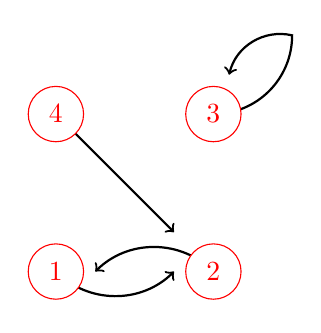
\begin{tikzpicture}
                \draw[->,thick] (0,0) to[bend right=45] (1.5,0);
                \draw[->,thick] (2,0) to[bend right=45] (0.5,0);
                \draw[->,thick] (2,2) to[bend right=45] (3,3) to[bend right=45] (2.2,2.5);
                \draw[->,thick] (0,2) to (1.5,0.5);
                
                \filldraw[red,fill=white] ( 0,0 ) circle (10pt) node {1};
                \filldraw[red,fill=white] ( 2,0 ) circle (10pt) node {2};
                \filldraw[red,fill=white] ( 2,2 ) circle (10pt) node {3};
                \filldraw[red,fill=white] ( 0,2 ) circle (10pt) node {4};
            \end{tikzpicture}
        }{}
    \item   \solution{ Many solutions. Example: ~\\

            Graph:
    
            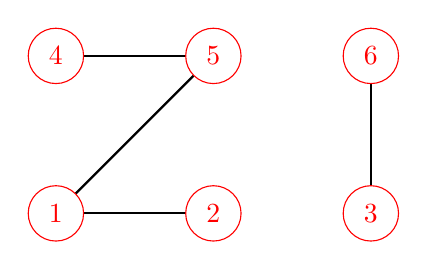
\begin{tikzpicture}
                \draw[thick] (0,0) -- (2,0);
                \draw[thick] (4,0) -- (4,2);
                \draw[thick] (0,0) -- (2,2);
                \draw[thick] (2,2) -- (0,2);
            
                \filldraw[red,fill=white] ( 0,0 ) circle (10pt) node {1};
                \filldraw[red,fill=white] ( 2,0 ) circle (10pt) node {2};
                \filldraw[red,fill=white] ( 4,0 ) circle (10pt) node {3};
                
                \filldraw[red,fill=white] ( 0,2 ) circle (10pt) node {4};
                \filldraw[red,fill=white] ( 2,2 ) circle (10pt) node {5};
                \filldraw[red,fill=white] ( 4,2 ) circle (10pt) node {6};
            \end{tikzpicture}

            Subgraph:
    
            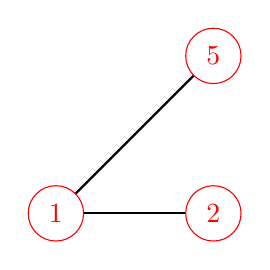
\begin{tikzpicture}
                \draw[thick] (0,0) -- (2,0);
                \draw[thick] (0,0) -- (2,2);
            
                \filldraw[red,fill=white] ( 0,0 ) circle (10pt) node {1};
                \filldraw[red,fill=white] ( 2,0 ) circle (10pt) node {2};
                
                \filldraw[red,fill=white] ( 2,2 ) circle (10pt) node {5};
            \end{tikzpicture}
        }{}
\end{enumerate}




\end{document}

